\subsubsection{Fahren mit weniger Informationen \dcfirstauthorshort}

Unser Algorithmus besteht im wesentlichen aus den zwei fusionierten Linienerkennungskomponenten Mittelstrich- und Randlinienerkennung. Um zu zeigen, dass diese nicht nur theoretisch unabhängig voneinander funktionieren, wurden zum Test je einmal die Mittellinie und die beiden Randlinien mit weißem Papier verdeckt. 

Da unser Algorithmus im wesentlichen aus den zwei nahezu unabhängigen, fusionierten Komponenten für die Mittelstrich- und die Randlinienerkennung besteht, soll in diesem Abschnitt gezeigt werden, dass 






\begin{figure}[htbp] % [htb]
	%\centering
	%\hfill
	\subfloat[Versuchsaufbau ohne Mittellinie \label{fig:evaluation:riverflow:ohneMittellinie:Versuchsaufbau}]{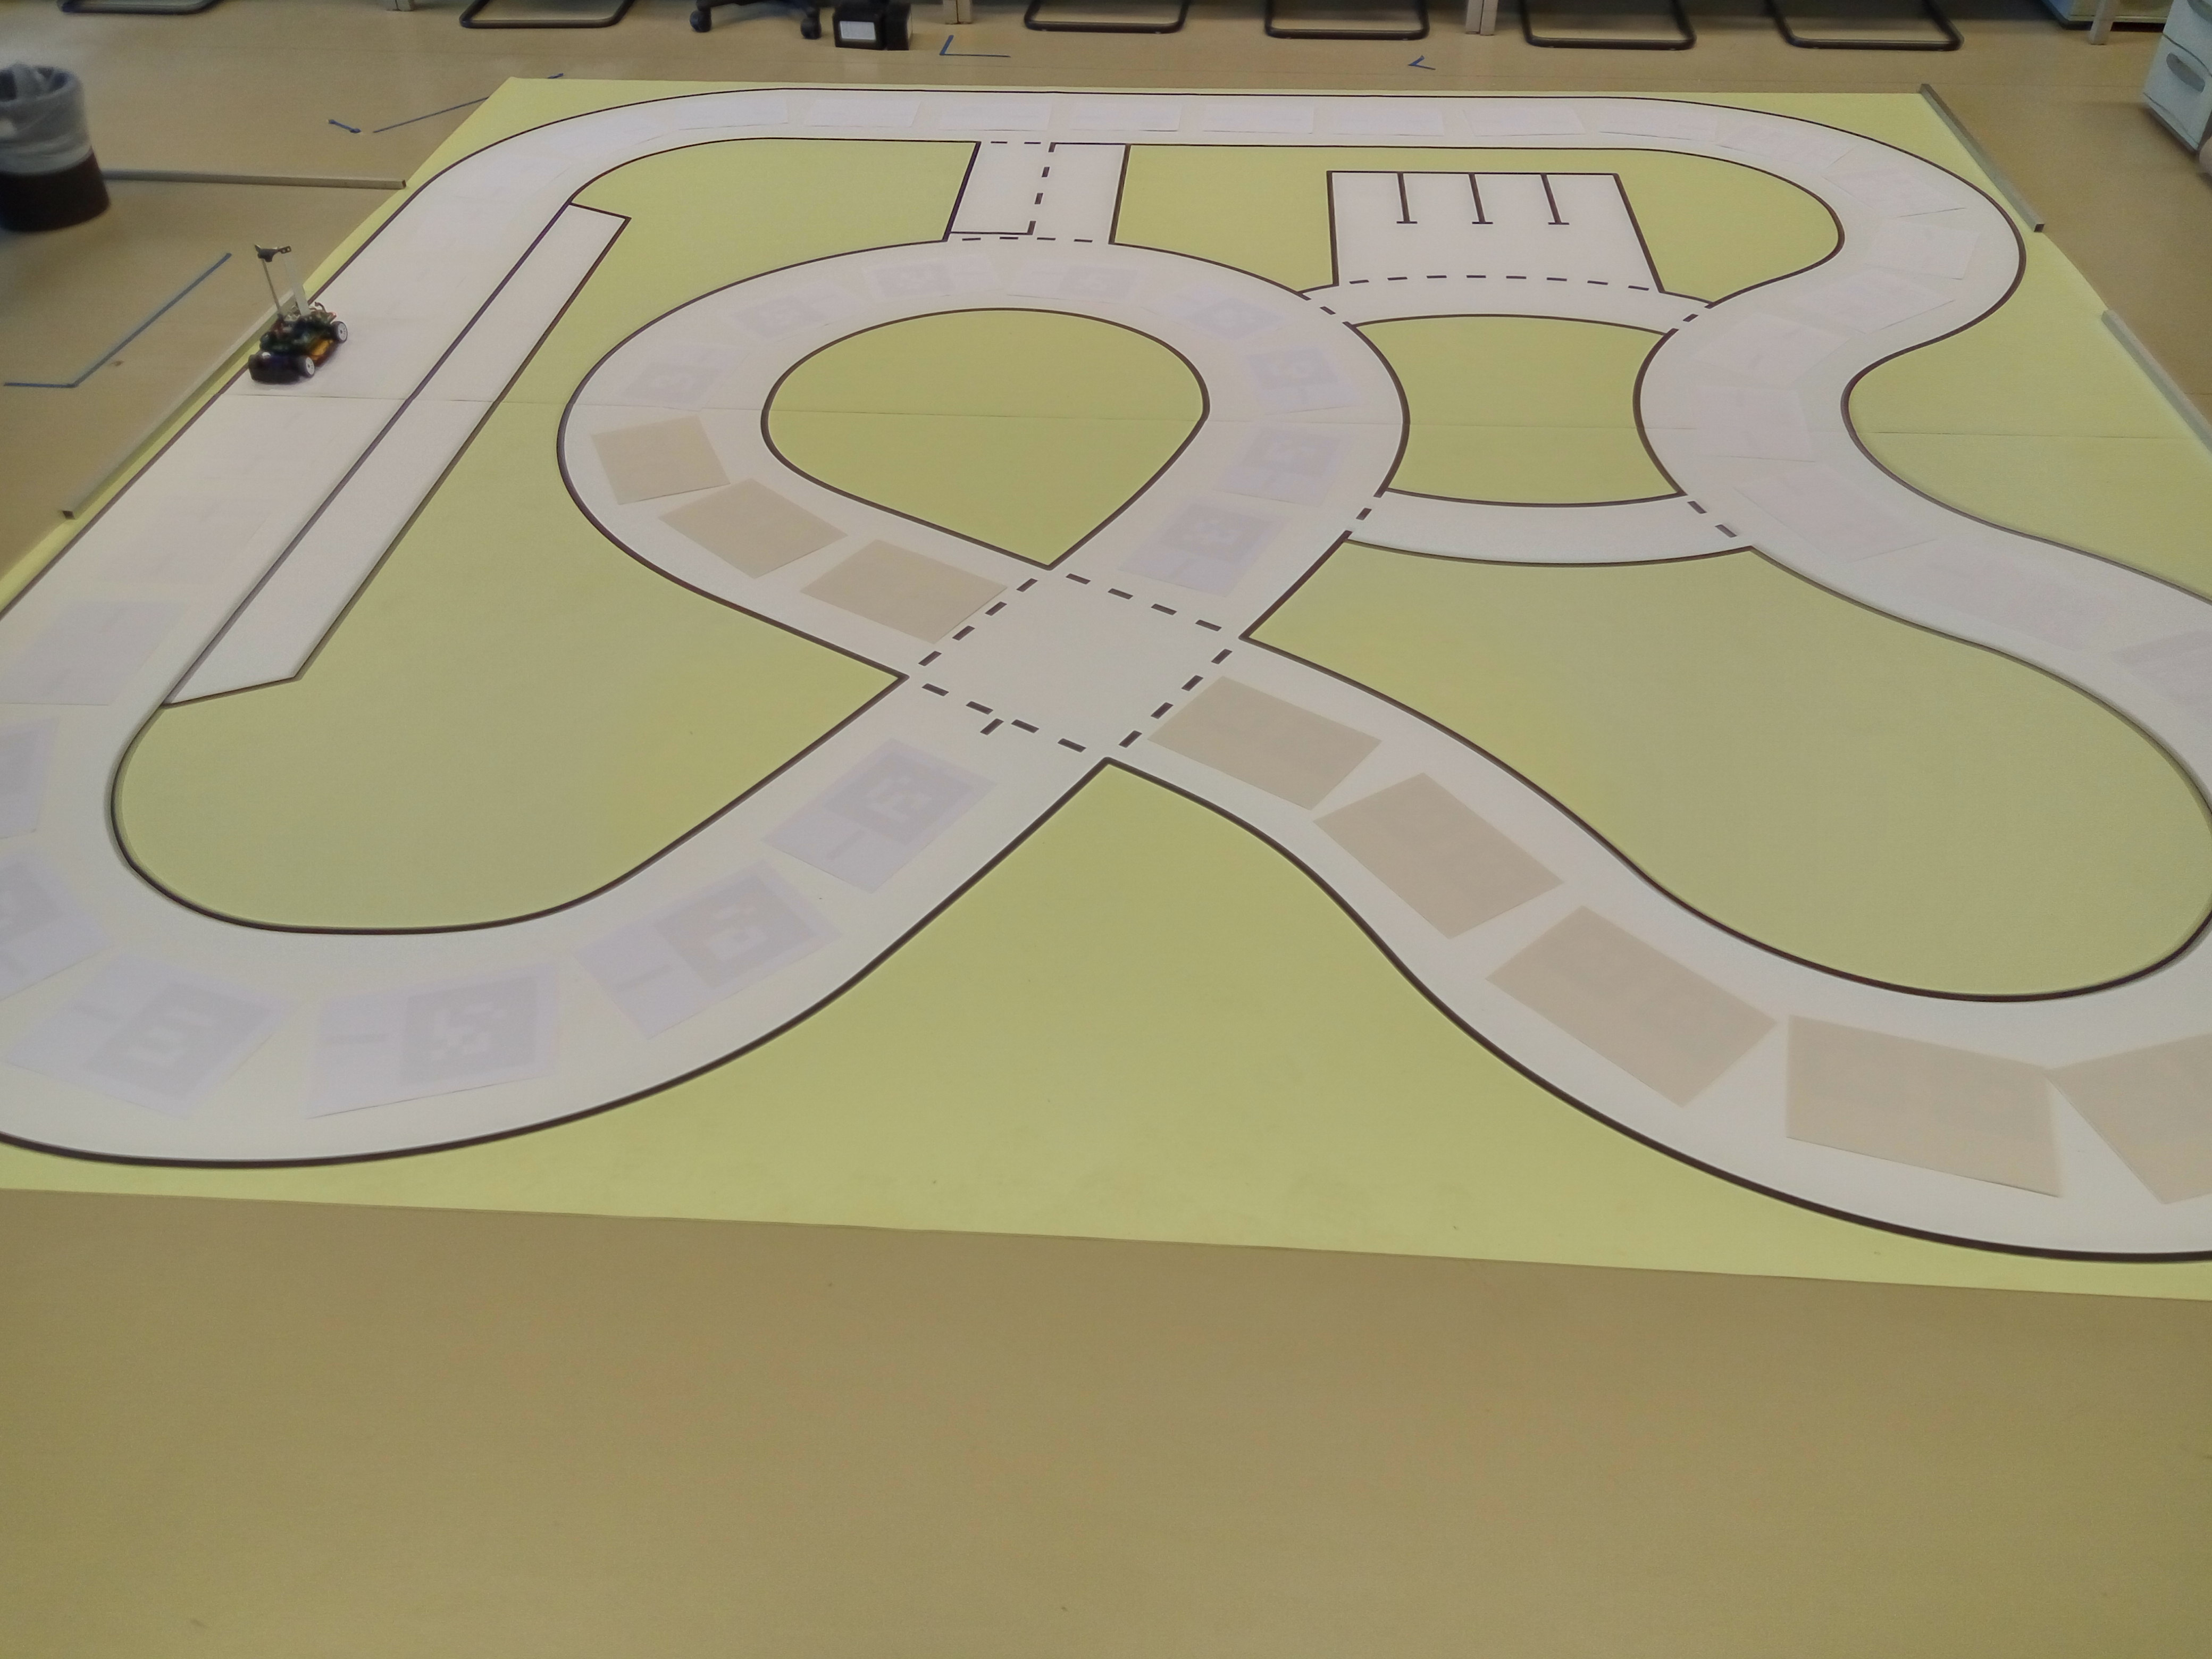
\includegraphics[width=0.49\textwidth]{evaluation_riverflow_ohne_mittellinie_versuchsaufbau.jpg}}
	\hfill
	\subfloat[Weltkarte ohne Mittellinie \label{fig:evaluation:riverflow:ohneMittellinie:Weltkarte}]{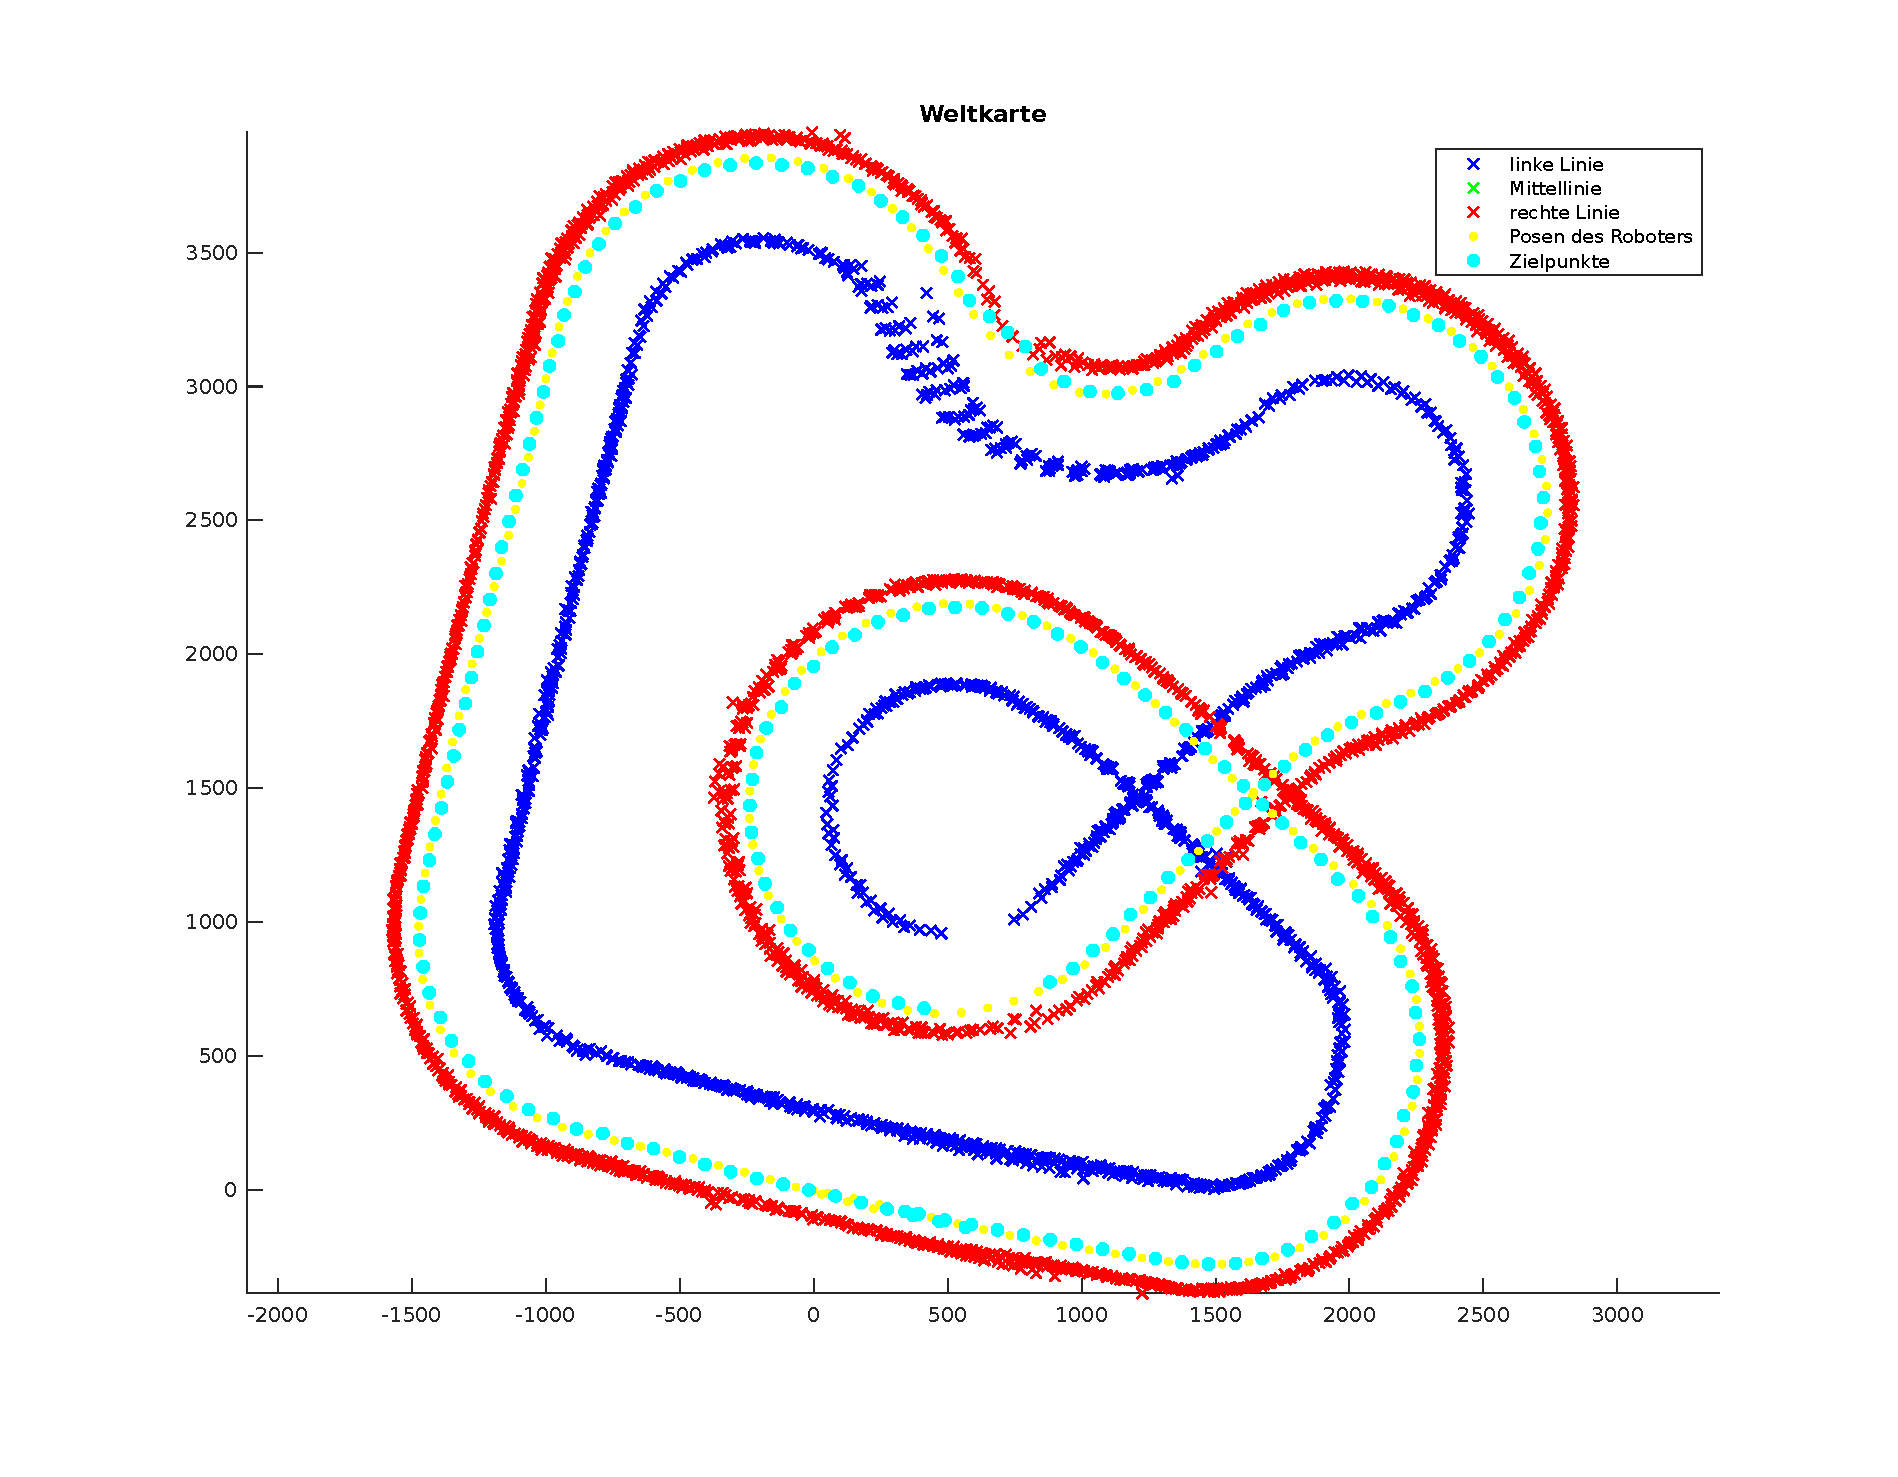
\includegraphics[width=0.49\textwidth]{evaluation_riverflow_ohne_mittellinie_worldmap.pdf}}
	\label{fig:evaluation:riverflow:ohneMittellinie}
	\caption{Testfahrt mit durch weißes Papier abgedeckte Mittelstriche}
\end{figure}



\begin{figure}[htbp] % [htb]
	\centering
	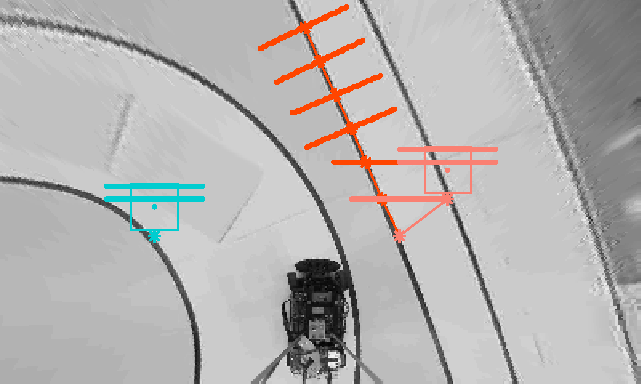
\includegraphics[width=0.7\textwidth]{evaluation_riverflow_ohne_mittellinie_problem_hough.pdf}
	\label{fig:evaluation:riverflow:ohneMittellinie:problem}
	\caption{Ungünstige Position für die mit Hough initialisierte Randlinienerkennung}
\end{figure}


\begin{figure}[htbp] % [htb]
	%\centering
	%\hfill
	\subfloat[Versuchsaufbau ohne Randlinien \label{fig:evaluation:riverflow:ohneRandlinie:Versuchsaufbau}]{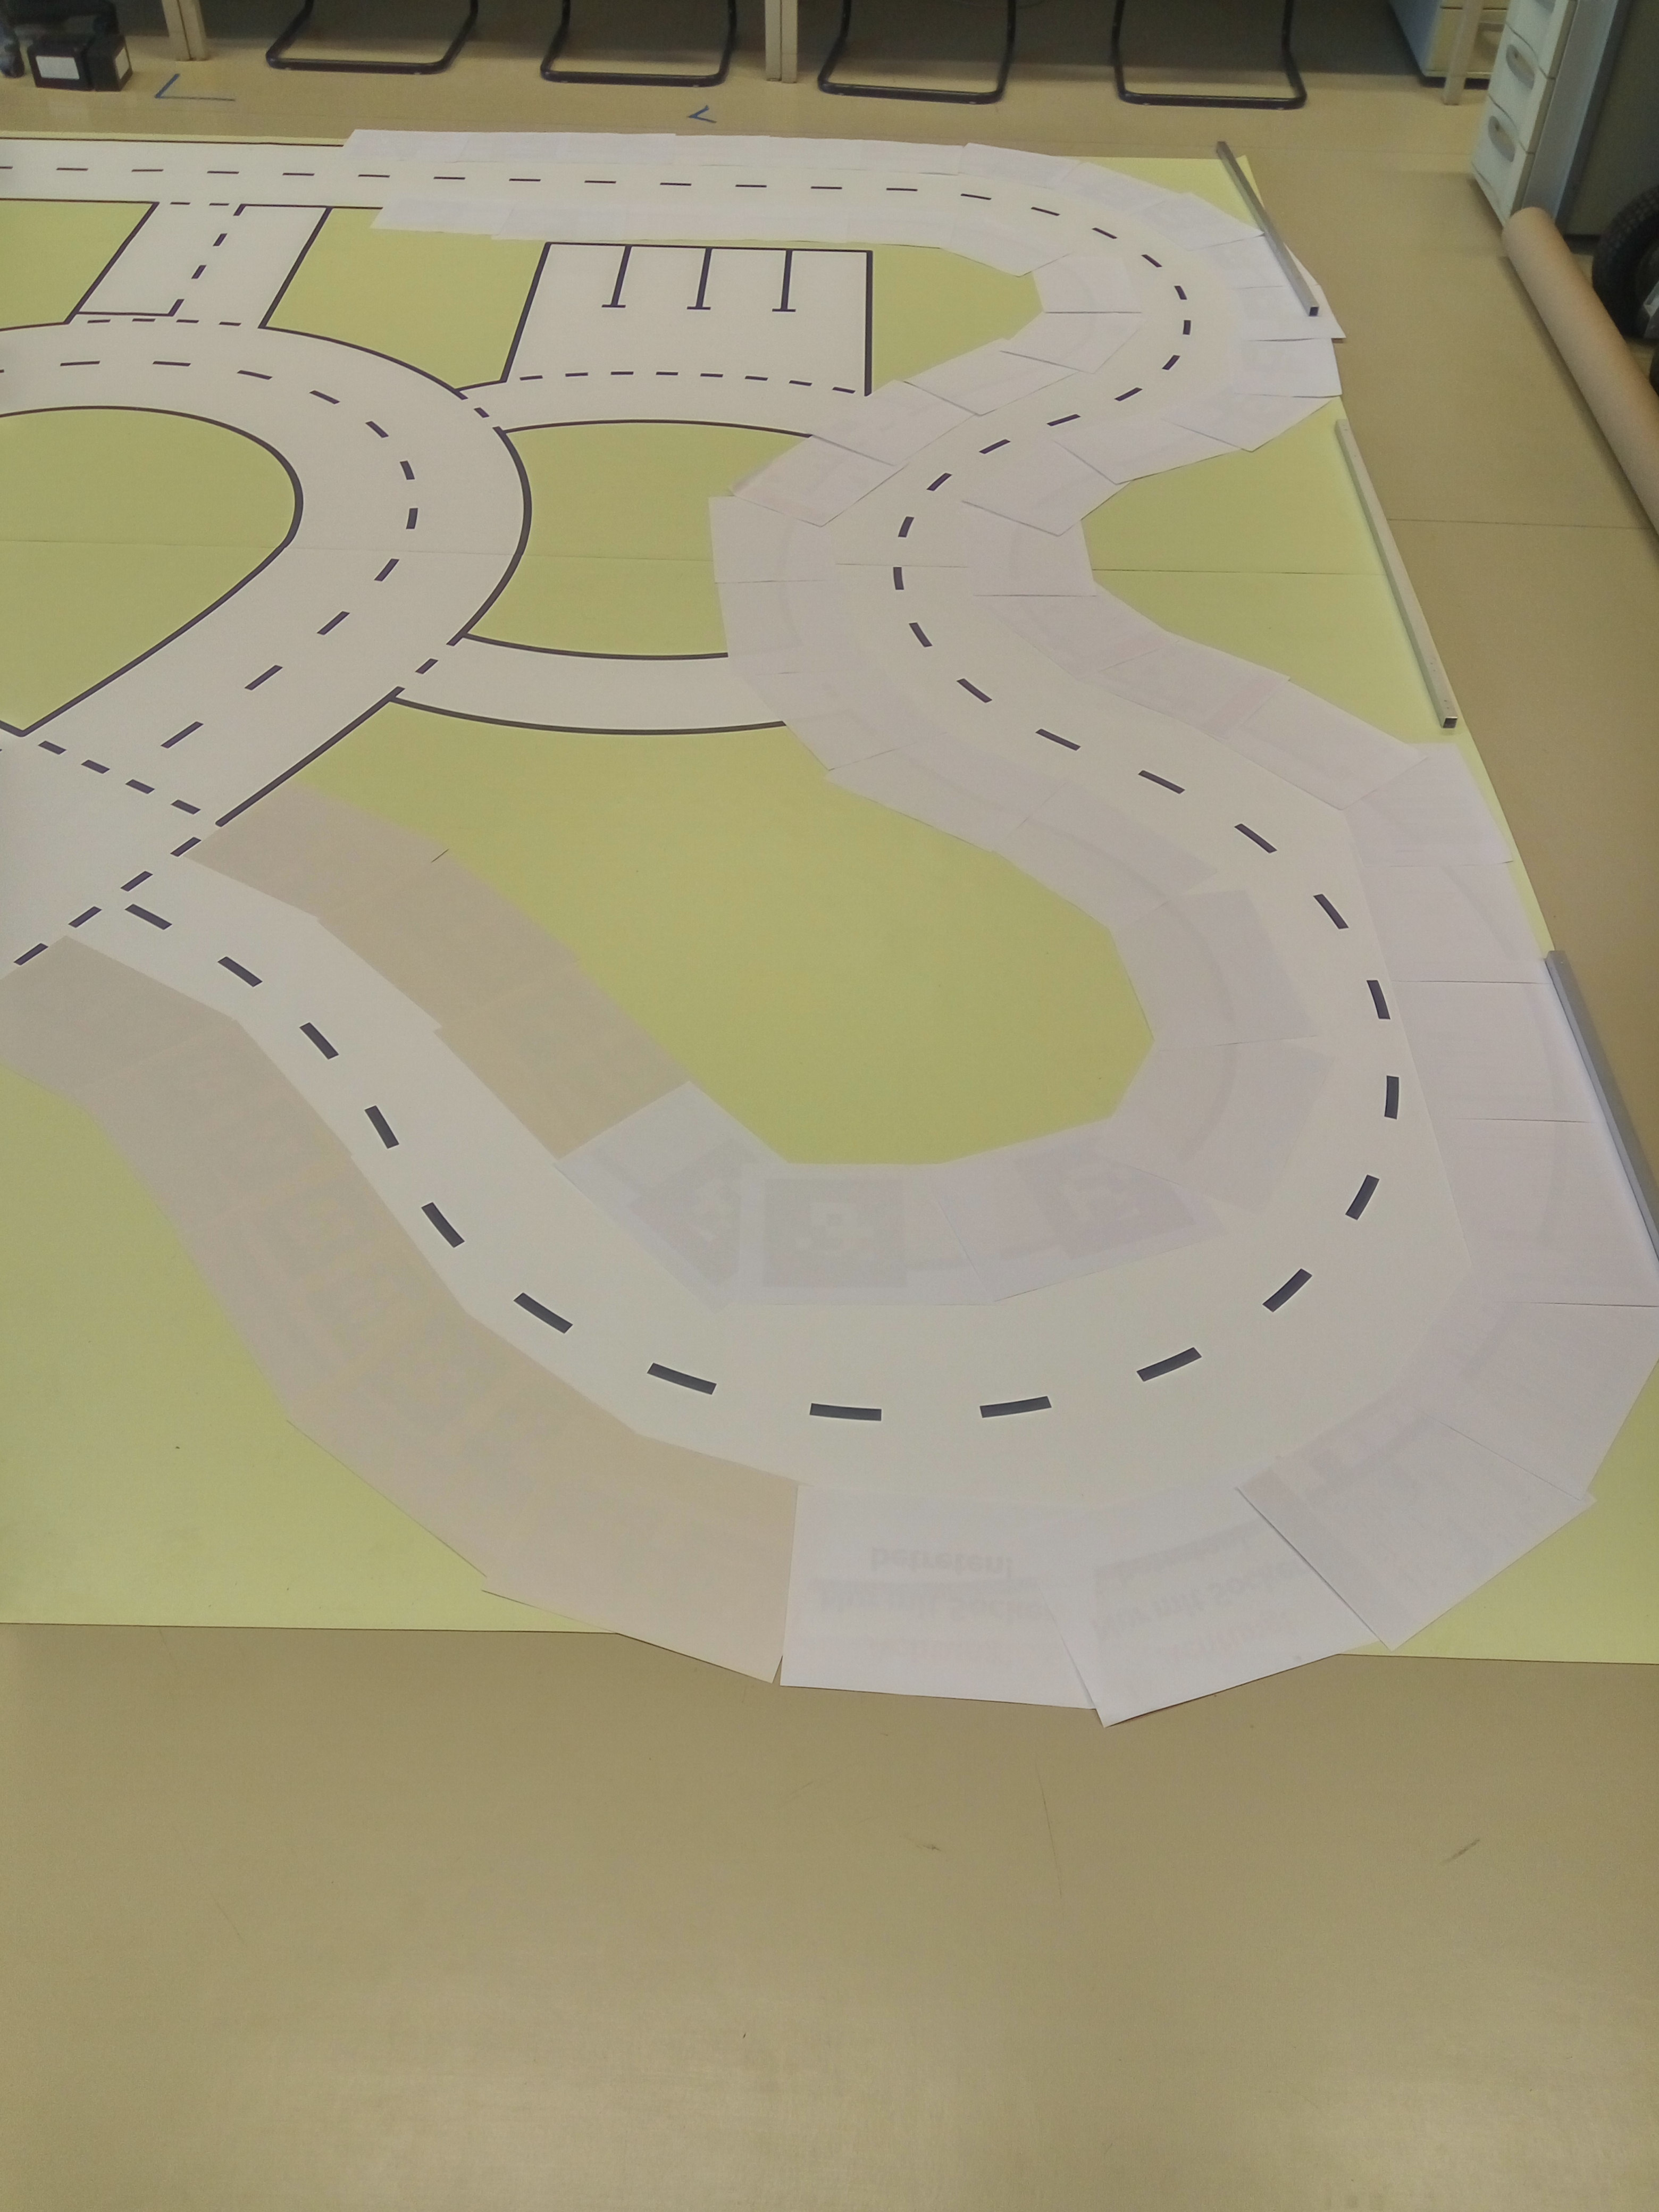
\includegraphics[width=0.49\textwidth]{evaluation_riverflow_ohne_randlinie_versuchsaufbau.jpg}}
	\hfill
	\subfloat[Weltkarte ohne Randlinien \label{fig:evaluation:riverflow:ohneRandlinie:Weltkarte}]{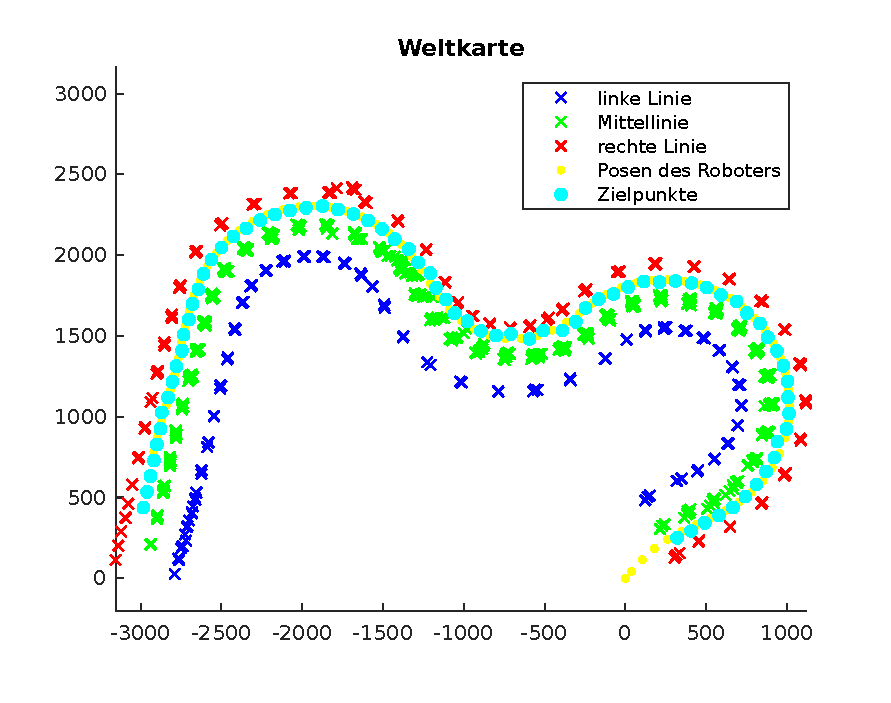
\includegraphics[width=0.49\textwidth]{evaluation_riverflow_ohne_randlinie_worldmap.pdf}}
	\label{fig:evaluation:riverflow:ohneRandlinie}
	\caption{Testfahrt mit durch weißes Papier abgedeckte Randlinien}
\end{figure}


\begin{figure}[htbp] % [htb]
	\centering
	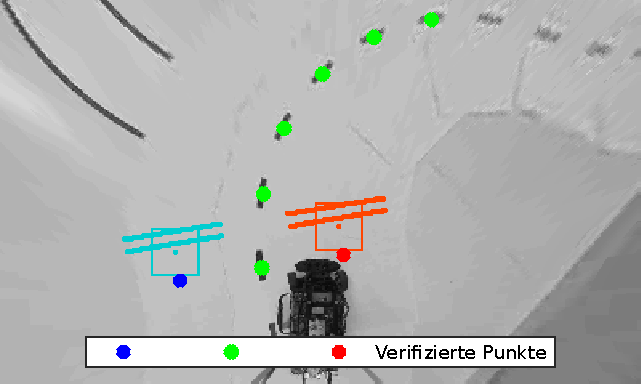
\includegraphics[width=0.7\textwidth]{evaluation_riverflow_ohne_randlinie_beispielplot.pdf}
	\label{fig:evaluation:riverflow:ohneMittellinie:bspPlot}
	\caption{Punkterkennung bei abgedeckten Randlinien}
\end{figure}





\begin{figure}[htbp] % [htb]
	%\centering
	%\hfill
	\subfloat[Beispielbild einer Unterbrechung \label{fig:evaluation:riverflow:Randlinie:unterbrochen:bsp}]{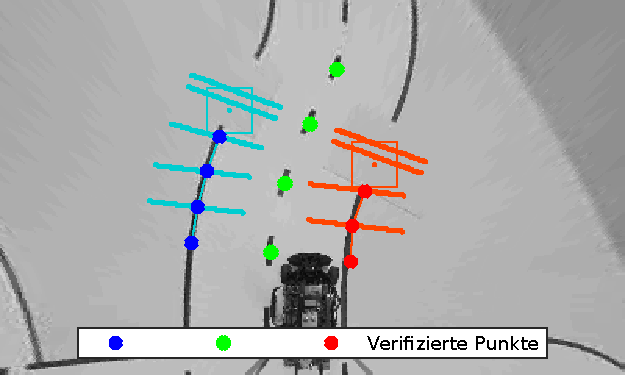
\includegraphics[width=0.49\textwidth]{evaluation_riverflow_randlinie_unterbrochen_beispiel.pdf}}
	\hfill
	\subfloat[Länge der erkannten Linien \label{fig:evaluation:riverflow:Randlinie:unterbrochen:linienlaenge}]{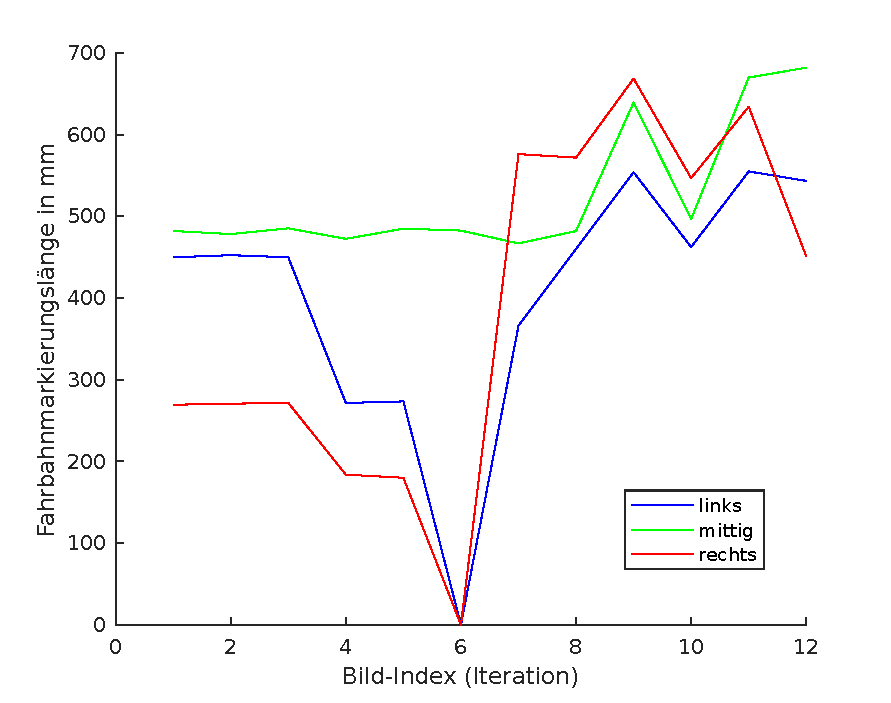
\includegraphics[width=0.49\textwidth]{evaluation_riverflow_randlinie_unterbrochen_plot_linienlaenge.pdf}}
	\label{fig:evaluation:riverflow:Randlinie:unterbrochen}
	\caption{Demonstration der Schwäche des Riverflow bei größeren Unterbrechungen in der Randlinie}
\end{figure}
